% THIS DOCUMENT IS FOLLOWS THE VOLERE TEMPLATE BY Suzanne Robertson and James Robertson
% ONLY THE SECTION HEADINGS ARE PROVIDED
%
% Initial draft from https://github.com/Dieblich/volere
%
% Risks are removed because they are covered by the Hazard Analysis
\documentclass[12pt]{article}

\usepackage{booktabs}
\usepackage{tabularx}
\usepackage{hyperref}
\usepackage{graphicx}
\hypersetup{
    bookmarks=true,         % show bookmarks bar?
      colorlinks=true,      % false: boxed links; true: colored links
    linkcolor=red,          % color of internal links (change box color with linkbordercolor)
    citecolor=green,        % color of links to bibliography
    filecolor=magenta,      % color of file links
    urlcolor=cyan           % color of external links
}

\newcommand{\lips}{\textit{Insert your content here.}}

\input{../Comments}
\input{../Common}

\begin{document}

\title{Software Requirements Specification for\\\progname}
\author{
    Team \#25, The Crazy Four \\[1ex]
    Ruida Chen \\
    Ammar Sharbat \\
    Alvin Qian \\
    Jiaming Li
}
\date{30.09.2025}
    
\maketitle

~\newpage

\pagenumbering{roman}

\tableofcontents

~\newpage

\section*{Revision History}

\begin{table}[hp]
    \caption{Revision History} \label{TblRevisionHistory}
    \begin{tabularx}{\textwidth}{llX}
        \toprule
        \textbf{Date} & \textbf{Developer(s)} & \textbf{Change}\\
        \midrule
        9.29 & Jiaming Li & 1 - Purpose of the Project\\
        9.30 & Ruida Chen & Section 3, 10 ,11,  12\\
        9.30 & Jiaming Li & 8 - Scope of the Product\\
        9.30 & Jiaming Li & 9 - Functional Requirements\\
        9.30 & Alvin Qian & Section 4,6,7\\
        10.1 & Alvin Qian & Section 14,16\\
        10.9 & Ruida Chen & Section 20,21,22\\
        10.9 & Jiaming Li & Section 17,18,19\\
        10.9 & Alvin Qian & Appendix and Reflection\\
        10.12 & Ammar Sharbat & Section 1.1, 2, 5, 13, 15, 18\\
        10.13 & Ammar Sharbat & Section 18, 19, 25\\
        04.06 & Ammar Sharbat & Section 1, 11, Removed Section 18\\
        04.07 & Ammar Sharbat & Section 2\\
        
        \bottomrule
    \end{tabularx}
\end{table}

~\\

~\newpage
\section{Purpose of the Project}
\subsection{User Business}
The purpose is to create an educational, game-based experience that introduces alternate number systems, especially dozenal, to learners who are currently more familiar with decimal arithmetic. The product will demonstrate the advantages of dozenal by embedding base-12 scoring and notation into a familiar card game structure, making abstract concepts concrete through gameplay.\\
\\
We aim to accomplish the aforementioned by designing and implementing an educational card game based on the traditional \textit{Crazy Eights} rule set, but with the following differences and additions:
\begin{itemize}
    \item Switching the wild card from ``8'' to ``10'' to highlight that the game uses alternate numeric notation: ``10'' in base-12 represents twelve in decimal, not ten.
    \item Incorporating counting into the game so players learn base conversion and divisibility in context.
    \item Integrating the \textbf{Dozenal (base-12)} number system into scoring, display, and feedback.
    \item Using a special \textbf{Dozenal (base-12)} deck of cards (with 4 standard suits, ranks 0--9, \rotatebox{180}{2}, \rotatebox{180}{3}, 10 and face cards J, Q, K, C).
\end{itemize}

\subsection{Goals of the Project}
The Minimum Viable Product (MVP) introduces dozenal (base-12) concepts through an engaging Crazy Eights card game, while laying the foundation for future educational expansions.

\subsubsection{MVP Functional Goals}
\begin{itemize}
    \item \textbf{Two-Player Core Loop:} Support a one-versus-one match with turn-taking, drawing, discarding, and win checks. Includes starter card, discard pile, and reshuffling the stock pile. \\
    \textbf{Rationale:} Two players are the smallest playable unit; finishing this proves the core loop.
    \item \textbf{Classic Rules Engine:} Implement standard Crazy Eights: match by suit or rank; an ``8'' is wild and lets the player declare a suit; draw if no valid move exists. \\
    \textbf{Rationale:} Correct classic rules establish a solid baseline before adding variations.
    \item \textbf{Dozenal (Base-12) Scoring/Display:} Display scores, counters, or thresholds in base-12 notation while keeping classic rules unchanged. \\
    \textbf{Rationale:} Introduces dozenal in a simple, non-disruptive way that highlights novelty while retaining accessibility.
\end{itemize}

\subsubsection{MVP Non-functional Goals}
\begin{itemize}
    \item \textbf{Move Validation and Feedback:} Provide immediate invalid-move feedback, clear suit selection UI after playing an ``8,'' and real-time state indicators. \\
    \textbf{Rationale:} Reduces errors and learning curve; improves usability.
    \item \textbf{Testability and Determinism:} Support seeded shuffling and provide basic logs or replays for each session. \\
    \textbf{Rationale:} Enables reproducible unit/integration testing and debugging.
    \item \textbf{Stability and Performance:} Ensure responsive UI $<200\,\text{ms}$, no crashes, no deadlocks, and correct reshuffling. \\
    \textbf{Rationale:} Reliability is the baseline for acceptance and live demonstration.
    \item \textbf{Minimal UI:} Provide a desktop or web interface showing hand, discard pile, current state, and a dozenal score tracker. \\
    \textbf{Rationale:} Covers essential interactions while limiting complexity at the MVP stage.
\end{itemize}

\subsubsection{Stretch Goals}
Stretch goals include extending the game to support more players, online multiplayer, AI opponents, advanced dozenal variants, and enhanced usability features such as tutorials and cross-platform deployment. These are detailed in the Waiting Room section.

\section{Stakeholders}

\subsection{Client}
\begin{itemize}
  \item \textbf{Professor Paul Rapoport, Mathematician} - paul.rapoport@mcmaster.ca. As a professor at McMaster University, he is responsible for the general direction, design decisions of the project, and concept mentorship.
  \item \textbf{Dr. Spencer Smith, Engineering Professor} - spencer.smith@mcmaster.ca. As a professor at McMaster University, he is responsible for project progress, deliverables, and development mentorship.
\end{itemize}

\subsection{Customer}
\begin{itemize}
  \item \textbf{Mathematicians:} Responsible for conceptual design decisions, ensuring the game's mathematical accuracy and educational value.
  \item \textbf{Educators:} Responsible for teaching aspects of the game and gameplay, including how it integrates into curricula and learning outcomes.
  \item \textbf{Students:} Responsible for the UI/web-game design and gameplay feedback, focusing on usability and engagement for their age group.
\end{itemize}

\subsection{Other Stakeholders}
\begin{itemize}
  \item \textbf{Other Scientists:} Provide expert input on alternative number systems and their applications, relating to use cases involving educational deployments and conceptual validation.
  \item \textbf{Parents and Children:} Offer feedback on family-friendly aspects, influencing deployments in home settings and casual learning scenarios.
  \item \textbf{Gamers:} Contribute to gameplay balance and fun factor, impacting use cases for recreational play and competitive modes.
  \item \textbf{Game Developers:} Advise on technical implementation and best practices, supporting deployments across different platforms and integrations.
  \item \textbf{General Public:} Represent broader societal interest, affecting use cases for public education and awareness campaigns.
\end{itemize}

\subsection{Hands-On Users of the Product}
\begin{itemize}
  \item \textbf{User name/category:} Students (ages 10-30). \\
  \textbf{User role:} Players who engage with the game for fun and learning. \\
  \textbf{Subject matter experience:} Novice - little to no prior knowledge of dozenal or alternative bases. \\
  \textbf{Technological experience:} Novice - basic computer skills, comfortable with web browsers. \\
  \textbf{Other user characteristics:} Ages 10-30, motivated by curiosity; may need simple tutorials; prefer visual and interactive elements.
  
  \item \textbf{User name/category:} Educators (teachers or instructors). \\
  \textbf{User role:} Facilitators who use the game in classroom settings. \\
  \textbf{Subject matter experience:} Journeyman - familiar with math education but may not know dozenal deeply. \\
  \textbf{Technological experience:} Journeyman - regular use of educational software and online tools. \\
  \textbf{Other user characteristics:} Ages 25-55, focused on pedagogical value; need exportable results and session management; value ease of setup.
  
  \item \textbf{User name/category:} Gamers. \\
  \textbf{User role:} Players who enjoy strategic card games and challenges. \\
  \textbf{Subject matter experience:} Journeyman - interested in learning new concepts through play. \\
  \textbf{Technological experience:} Master - experienced with online games and interfaces. \\
  \textbf{Other user characteristics:} Ages 5-40, competitive; appreciate fair rules and replay features; tolerant of brief learning curves.
  
  \item \textbf{User name/category:} Capstone Evaluators (professors or experts). \\
  \textbf{User role:} Assessors who evaluate the project's technical and educational merits. \\
  \textbf{Subject matter experience:} Master - deep expertise in software engineering and math education. \\
  \textbf{Technological experience:} Master - proficient in various development tools and platforms. \\
  \textbf{Other user characteristics:} Ages 30-60, analytical; focus on correctness, stability, and scalability; provide detailed feedback.
  
  \item \textbf{User name/category:} Parents. \\
  \textbf{User role:} Supervisors who introduce the game to children at home. \\
  \textbf{Subject matter experience:} Novice to journeyman - basic math knowledge, supportive of learning. \\
  \textbf{Technological experience:} Journeyman - regular internet users, comfortable with family apps. \\
  \textbf{Other user characteristics:} Ages 25-50, concerned with safety and appropriateness; prefer guided experiences for kids.
  
  \item \textbf{User name/category:} Children (young learners). \\
  \textbf{User role:} Young players exploring math through games. \\
  \textbf{Subject matter experience:} Novice - early math exposure, curious about numbers. \\
  \textbf{Technological experience:} Novice - learning to use devices, enjoy interactive content. \\
  \textbf{Other user characteristics:} Ages 8-14, playful; need simple, colorful interfaces; short attention spans.
\end{itemize}

\subsection{Personas}

\subsubsection{Educators / Instructors}

\includegraphics[width=1\textwidth]{Personas/elena_ramirez.jpg} \\
\textbf{Elena Ramirez, 42-year-old High School Math Teacher:} Elena is a dedicated educator at a local high school, passionate about making math engaging for her students. She discovered dozenal through a professional development workshop and sees it as a way to challenge traditional teaching methods. In her daily life, she spends hours planning lessons, grading papers, and attending parent-teacher meetings. Elena uses educational apps to supplement her classroom activities and is always looking for innovative tools to spark student interest. She dreams of inspiring the next generation of mathematicians and enjoys hiking and reading science fiction in her free time. For this project, Elena would provide feedback on how the game fits into curricula and helps students grasp alternative number systems.

\subsubsection{Students / Casual Learners}

\includegraphics[width=1\textwidth]{Personas/alex_chen.jpg} \\
\textbf{Alex Chen, 16-year-old High School Student:} Alex is a curious teenager who loves puzzles and games but finds traditional math classes boring. He stumbled upon dozenal while browsing online and became fascinated by how it could simplify fractions. As a student, Alex juggles schoolwork, extracurricular activities like the chess club, and hanging out with friends. He spends a lot of time on his phone playing mobile games and watching educational YouTube videos. Alex is tech-savvy, preferring intuitive apps over complicated software. He hopes to pursue engineering in college and sees learning dozenal as a fun way to build his problem-solving skills. For this project, Alex would test the game's usability and suggest improvements to make it more engaging for peers his age.

\subsubsection{Gamers / General Public}
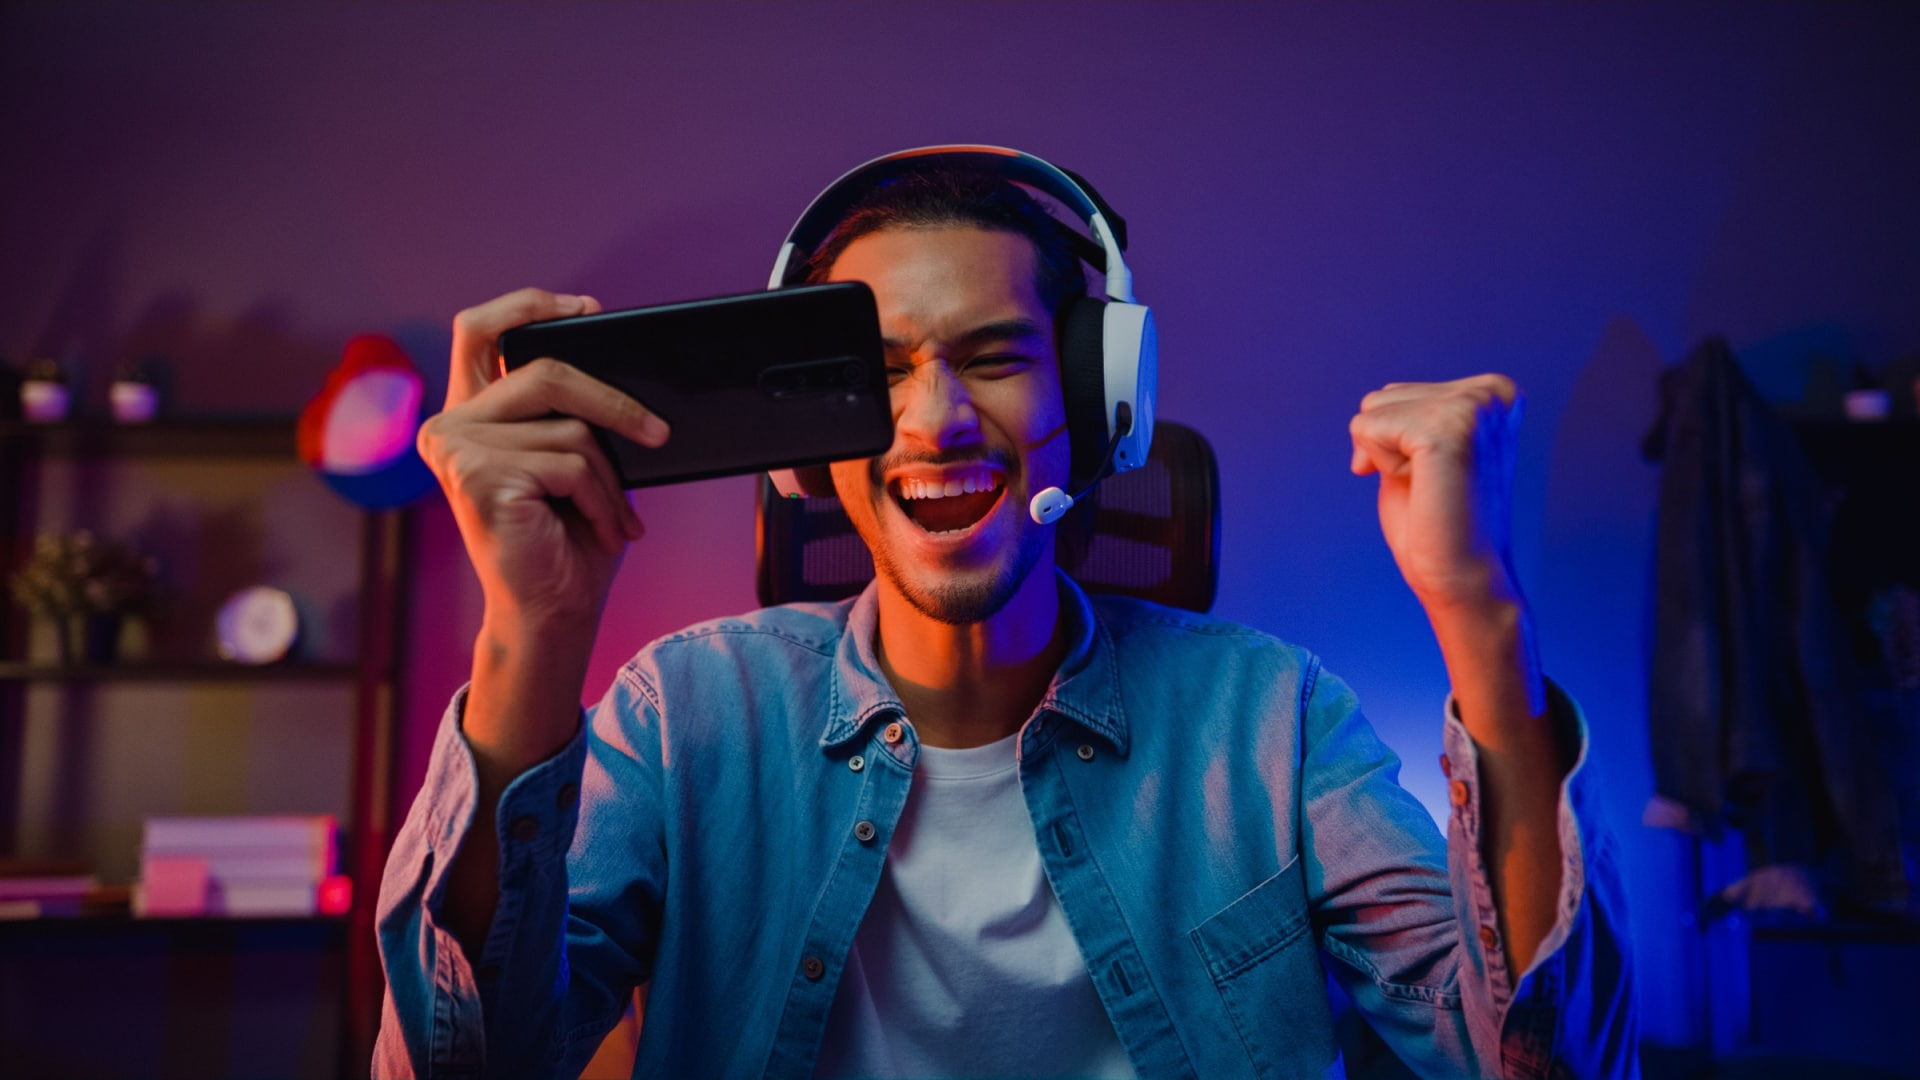
\includegraphics[width=1\textwidth]{Personas/mike_torres.jpg} \\
\textbf{Mike Torres, 28-year-old Software Developer and Casual Gamer:} Mike works as a software developer by day, coding and debugging applications, but unwinds by playing card games and strategy titles online. He came across dozenal in a forum discussion about efficient number systems and thought it could make for an interesting game mechanic. In his life, Mike balances work deadlines, gym sessions, and gaming nights with friends. He's active in online gaming communities, sharing tips and reviewing new releases. Mike values fair gameplay and innovative features that add depth without complexity. He enjoys learning new concepts through entertainment and often researches game design. For this project, Mike would evaluate the game's balance, provide technical feedback, and suggest ways to appeal to the broader gaming audience.

\subsection{Priorities Assigned to Users}
\begin{itemize}
  \item \textbf{Key users:}
    \begin{itemize}
      \item Educators - they are the primary facilitators of the educational aspect and will integrate the game into learning environments.
      \item Students - they are the main audience for the educational content and will provide critical feedback on usability and engagement.
    \end{itemize}
  
  \item \textbf{Secondary users:}
    \begin{itemize}
      \item Capstone evaluators - they provide expert feedback on conceptual validity and educational value, influencing design decisions and future enhancements.
      \item Parents and children - they represent the family audience and provide insights on accessibility and appeal for younger users, impacting use cases for home learning and casual play.
      \item Mathematicians and Scientists - they contribute to the broader scientific context and potential applications of dozenal, influencing use cases for public education and awareness.
      \item Gamers - they offer feedback on gameplay mechanics and balance, affecting use cases for recreational play and competitive modes.
    \end{itemize}
    These users are secondary as they provide valuable feedback during testing and demos, helping refine the product, but they are not the core audience for daily use.
  
  \item \textbf{Unimportant users:}
    \begin{itemize}
      \item Educational Institutions - while they influence many of the other stakeholders, they are not directly involved in the design or feedback process.
      \item Game Developers - they may provide technical advice but are not the end users or primary evaluators of the educational content.
      \item General public / Anonymous spectators - they may have general interest but do not actively participate in the design or feedback process.
    \end{itemize}
    These users are considered unimportant in terms of priority because, while they contribute to broader impact and family engagement, they have less direct involvement in the core functionality and decision-making processes.
\end{itemize}

\subsection{User Participation}
\begin{itemize}
  \item \textbf{Educators:} Estimated 2-4 hours over the term for reviewing tutorial content and alignment with learning objectives; provide knowledge on pedagogical effectiveness and curriculum integration.
  \item \textbf{Students:} Estimated 3-5 sessions of 20-30 minutes for playtesting; provide knowledge on usability, engagement, and age-appropriate design.
  \item \textbf{Demonstration evaluators} Estimated 2-3 hours per month for feedback sessions; provide feedback on overall project / game progess and design and development.
  \item \textbf{Mathematicians Scientists:} Estimated 1-2 hours for content review; provide knowledge on mathematical accuracy and conceptual depth.
  \item \textbf{Parents and children:} Estimated 30 minutes - 1 hour for family testing; provide knowledge on accessibility and family-friendly features.
  \item \textbf{Gamers:} Estimated 10-20 minute sessions for gameplay testing; provide knowledge on game balance and competitive elements.
  \item \textbf{General Public and Anonymous spectators} Minimal participation; provide general impressions if surveyed.
\end{itemize}

\subsection{Maintenance Users and Service Technicians}
\begin{itemize}
  \item \textbf{Computer Scientists:} Responsible for ongoing system maintenance, updates, and troubleshooting technical issues; they ensure the software remains functional and secure over time.
  \item \textbf{Game Developers:} Handle content updates, bug fixes, and feature enhancements; they maintain the game's integrity and adapt it to new platforms or user needs.
\end{itemize}

\subsubsection*{Fit criterion}
Stakeholder list and contact/role assignments exist in the project README and team Kanban; at least one named representative for each stakeholder category is recorded. Evidence: README / Team Roles section and meeting minutes indicating stakeholder reviews.


\section{Mandated Constraints}

\subsection{Solution Constraints}
\textbf{Description:} The system must be developed using a sound and scalable technology stack that supports web-based deployment.
\textbf{Rationale:} Ensures the team gains proficiency in useful modern web development frameworks, aligning with the project's educational goals and contributing to long-term career growth. These technologies provide strong essential knowledge for building robust web applications.
\textbf{Fit Criterion:} The frontend code is written in React (verified by package.json and component structure), and the backend is implemented in Node.js (verified by server files and runtime environment).

\textbf{Description:} All source code must be managed using version control, with frequent commits, issue tracking and project management.
\textbf{Rationale:} Version control is essential for collaborative development, and maintaining a history of changes, which is critical for team coordination and project traceability.
\textbf{Fit Criterion:} All code is stored in a GitHub repository, with commits made for each significant change and pull requests used for code reviews.

\subsection{Implementation Environment of the Current System}

\textbf{Server-hosting:} The backend must operate with a consistent server side connection.
\textbf{Rationale:} A stable server environment is essential for hosting the game logic, managing user sessions, and ensuring real-time interactions between players.
\textbf{Fit Criterion:} The application runs on Node.js LTS and connects to a relational database, as confirmed by deployment and testing in the specified environment.

\textbf{Data Management:} The system must sustain user data and game statistics.
\textbf{Rationale:} Persistent data storage is essential for tracking user progress, game history, and providing a personalized experience.
\textbf{Fit Criterion:} Using a relational database such as PostgreSQL or MySQL with defined schemas for users, games, and scores.

\textbf{Browser Compatibility:} The application must be deployable on modern web browsers (Chrome, Firefox, Edge).
\textbf{Rationale:} Targeting modern browsers ensures broad accessibility and compatibility with standard web technologies.
\textbf{Fit Criterion:} The application loads and functions correctly in Chrome, Firefox, and Edge, verified through cross-browser testing.

\subsection{Partner or Collaborative Applications}

\textbf{Description:} The team must use GitHub for code collaboration and issue tracking.
\textbf{Rationale:} GitHub facilitates distributed development and project management through its integrated tools.
\textbf{Fit Criterion:} All team members use GitHub for code pushes, issue creation, and project tracking.

\textbf{Description:} Discord is required for real-time communication and coordination.
\textbf{Rationale:} Discord provides efficient channels for quick updates, discussions, and meetings, supporting remote collaboration.
\textbf{Fit Criterion:} Team communications occur via Discord channels, with records of key decisions logged.

\subsection{Off-the-Shelf Software}

\textbf{Description:} The system must rely primarily on open-source libraries.
\textbf{Rationale:} Open-source libraries reduce costs and promote community-supported, reliable components.
\textbf{Fit Criterion:} All third-party libraries used are open-source, as listed in package.json or equivalent dependency files.

\textbf{Description:} Proprietary software must not be required for end users to run the application.
\textbf{Rationale:} Ensuring no proprietary dependencies allows free access and broad usability.
\textbf{Fit Criterion:} The application runs without requiring any proprietary software installations, verified by user testing.

\subsection{Anticipated Workplace Environment}

\textbf{Description:} End users are expected to interact with the application primarily on web browsers.
\textbf{Rationale:} Web-based deployment simplifies access and reduces platform-specific requirements.
\textbf{Fit Criterion:} The application is fully functional within web browsers without additional software.

\subsection{Schedule Constraints}

\textbf{Description:} The project must be completed within the academic deadline.
\textbf{Rationale:} Academic timelines ensure timely delivery and alignment with course requirements.
\textbf{Fit Criterion:} All deliverables are submitted by the specified deadlines, as per the project schedule.

\textbf{Description:} Progress reports and milestone check-ins with the TA are mandatory.
\textbf{Rationale:} Regular check-ins provide oversight and feedback to maintain project quality.
\textbf{Fit Criterion:} Check-ins occur as scheduled, with documented progress and TA approvals.

\subsection{Budget Constraints}

\textbf{Description:} Total financial budget is under 500 Canadian Dollars.
\textbf{Rationale:} Limited budget enforces cost-effective development using free or low-cost tools.
\textbf{Fit Criterion:} All project expenses remain under 500 CAD, tracked via receipts and logs.

\textbf{Description:} Open-source and free tools are primarily to be used.
\textbf{Rationale:} Free tools minimize costs and promote sustainable development practices.
\textbf{Fit Criterion:} All development tools and services are free or open-source, confirmed by usage logs.

\subsection{Enterprise Constraints}

\textbf{Description:} The project must comply with academic integrity and university policies.
\textbf{Rationale:} Compliance ensures ethical development and avoids penalties.
\textbf{Fit Criterion:} All work adheres to university policies, verified through self-assessment and TA review.

\textbf{Description:} Data collection and storage must follow privacy, security, and ethical guidelines.
\textbf{Rationale:} Protecting user data builds trust and meets legal standards.
\textbf{Fit Criterion:} Data handling complies with privacy laws (e.g., no unauthorized data collection), audited via code review.


\section{Naming Conventions and Terminology}
\subsection{Glossary of All Terms, Including Acronyms, Used by Stakeholders
involved in the Project}

\begin{itemize}
    \item \textbf{Base-10 (Decimal)}: The standard numerical system using ten digits (0--9), commonly used in arithmetic and everyday calculations.
    \item \textbf{Base-12 (Dozenal)}: A numerical system using twelve digits (0--9, \reflectbox{2}, \reflectbox{3}), where \reflectbox{2} represents 10 and \reflectbox{3} represents 11 in decimal. Has divisibility advantages (divisors: 2, 3, 4, 6).
    \item \textbf{Base-8 (Octal)}: A numerical system using eight digits (0--7). Each octal digit represents three binary digits (bits). Commonly used in computing and digital systems due to easy conversion with binary.
    \item \textbf{Base-16 (Hexadecimal)}: A numerical system using sixteen digits (0--9, A--F), where A through F represent decimal values 10 to 15. Widely used in programming and computer memory addressing for its compact binary representation.
    \item \textbf{Crazy Eights}: A classic card game where players match cards by suit or rank, with the ``8'' card acting as a wild card allowing the player to declare a new suit.
    \item \textbf{MVP}: Minimum Viable Product, the initial version of the Crazy Eights software with core functionality, including two-player gameplay, classic rules, and dozenal scoring.
    \item \textbf{Functional Goals}: Features and behaviors the software must implement, such as gameplay mechanics and dozenal score display.
    \item \textbf{Non-functional Goals}: Quality attributes of the software, such as usability, performance, and stability.
    \item \textbf{Stretch Goals}: Optional features or enhancements, such as multiplayer support or advanced dozenal rule variants, to be implemented if time permits.
    \item \textbf{GitHub}: The platform used for version control, issue tracking, and Kanban board management.
    \item \textbf{Discord}: The communication platform for team coordination, quick updates, and voice meetings.
    \item \textbf{Kanban Board}: A project management tool in GitHub Projects, divided into stages (Backlog, In Progress, Review, Done) to track tasks.
    \item \textbf{CI/CD}: Continuous Integration/Continuous Deployment, an automated process for testing and deploying code changes.
    \item \textbf{SRS}: Software Requirements Specification, this document outlining the requirements for the Crazy Eights project.
    \item \textbf{PoC}: Proof of Concept, a prototype demonstrating core gameplay mechanics to validate feasibility.
    \item \textbf{UI}: User Interface, the visual and interactive components of the software, such as the game board and score display.
\end{itemize}

\section{Relevant Facts and Assumptions}

\subsection{Relevant Facts}
\begin{itemize}
  \item \textbf{Prevalence of decimal:} Users are overwhelmingly familiar with base-10; dozenal notation is novel for most.
  \item \textbf{Educational effectiveness:} Game-based learning improves numeracy engagement (backed by pedagogical literature).
  \item \textbf{Resource constraints:} Project budget is capped at 500 CAD and timeline is an academic term.
  \item \textbf{Technology stack:} Planned stack is React (frontend), Node.js (backend), PostgreSQL (data).
  \item \textbf{Browser target:} Modern desktop browsers (Chrome, Firefox, Edge) are the primary runtime environment.
\end{itemize}

\subsection{Business Rules}
\begin{itemize}
  \item \textbf{Scoring rule:} Round score equals sum of opponents' remaining card values (displayed in both decimal and dozenal).
  \item \textbf{Account rule:} Registered usernames must be unique; guest mode creates impermanent sessions.
  \item \textbf{Open-source rule:} All deliverables must use appropriately licensed assets; avoid proprietary-only dependencies.
\end{itemize}

\subsection{Assumptions}
\begin{itemize}
  \item \textbf{Connectivity:} Players typically have a stable internet connection for multiplayer sessions.
  \item \textbf{Device:} Primary devices are desktop/laptop; mobile support is a stretch-goal.
  \item \textbf{Play familiarity:} Players understand basic card game mechanics (matching suit or rank).
  \item \textbf{Team availability:} Team members will perform peer review before merges as per Development Plan.
  \item \textbf{Third-party components:} Standard open-source libraries (React, Socket.io, PG client) will be available and compatible.
\end{itemize}

\section{The Scope of the Work}
\subsection{The Current Situation}

No pre-existing educational card game exists that integrates Dozenal (Base-12) scoring and notation into gameplay to teach alternative number systems. Existing card games like Crazy Eights use decimal scoring, and educational tools for dozenal are limited to abstract calculators or texts, lacking interactive, gamified experiences that could engage learners and demonstrate practical advantages.

\subsection{The Context of the Work}

The work context focuses on the educational and recreational use of card games to teach alternative number systems. Adjacent systems include:

- Educational institutions (providing curriculum integration and student access).
- Math communities and academics (supplying feedback on dozenal concepts).
- Online desktop gaming platforms (providing gameplay data and engagement metrics).
- Web browsers and devices (enabling access to the game).

Inputs: User login data, game start requests, move inputs. Outputs: Game states, scores in dozenal, educational feedback.

This context ensures the product fits into learning environments without disrupting existing workflows.

\subsection{Work Partitioning}

The work is partitioned into business events and their corresponding business use cases (BUCs):
\begin{itemize}
  \item \textbf{BUC:  Game Initiation} - Triggered by user request to start a game.\\ Initialize Game Session. Outputs: Shuffled deck, dealt hands.
  \item \textbf{BUC:  Player Move} - Triggered by player selecting a card.\\ Process Move. Outputs: Updated game state, feedback.
  \item \textbf{BUC:  Game End} - Triggered when a player empties their hand.\\ Calculate and Display Score. Outputs: Final scores in dozenal.
  \item \textbf{BUC:  Educational Query} - Triggered by user requesting dozenal explanations.\\Provide Learning Resources. Outputs: Tutorials or hints.
\end{itemize}

\subsection{Specifying a Business Use Case (BUC)}

\textbf{BUC: Play a Game of Crazy Eights with Dozenal Scoring}

\begin{itemize}
    \item \textbf{Actors}: Two players, the software system.
    \item \textbf{Trigger}: A player creates a new game session using the UI.
    \item \textbf{Description}: Two players take turns matching cards by suit or rank, with the ``10'' card acting as a wild card that allows the player to declare a new suit. If no valid move can be made, the player draws from the stock pile. The game ends when one player discards all their cards, and the score is calculated and displayed in dozenal notation.
    \item \textbf{Preconditions}: The user is logged in. The software is running on a web interface, with a functional UI displaying the hand, discard pile, stock pile, and score tracker.
    \item \textbf{Postconditions}: The game concludes with a winner, points are displayed in dozenal and must be counted by the users to see the final score. The user can log Off or start a new game.
    \item \textbf{Basic Flow}:
    \begin{enumerate}
        \item The system deals cards to both players and initializes the discard pile with a starter card.
        \item Players take turns, selecting a card to play (matching suit or rank) or drawing from the stock pile.
        \item If an ``10'' is played, the player selects a new suit via the UI.
        \item The system checks moves and gives immediate feedback for invalid moves.
        \item The game keeps going until one player has no cards left, triggering user score counting and calculation challenge in dozenal.
        \item The system displays the final score.
    \end{enumerate}
    \item \textbf{Exceptions}:
    \begin{itemize}
        \item Invalid move attempted: The system highlights the error and prompts the player to select a valid card or draw.
        \item Stock pile exhausted: The system reshuffles the discard pile to replenish the stock pile.
    \end{itemize}
    \item \textbf{Assumptions}: Players are familiar with basic card game mechanics and the system supports a stable internet connection for play.
\end{itemize}

\section{Business Data Model and Data Dictionary}
\subsection{Business Data Model}

These are the key entities and relationships involved in the Crazy Eights game with dozenal scoring.

\begin{itemize}
    \item \textbf{Entities}:
    \begin{itemize}
        \item \textbf{Player}: Represents a game participant, holding a hand of cards and a score.
        \item \textbf{Card}: Represents a single playing card with a suit and rank.
        \item \textbf{Deck}: A collection of cards, divided into the stock pile and discard pile.
        \item \textbf{Game Session}: Tracks the state of a single game, including players, current turn, discard pile, and scores.
        \item \textbf{Score}: Tracks points in dozenal notation, calculated based on game rules.
    \end{itemize}
    \item \textbf{Relationships}:
    \begin{itemize}
        \item A \textbf{Game Session} has 2 \textbf{Players} (MVP) or 2--4 \textbf{Players} (stretch goal).
        \item Each \textbf{Player} has a \textbf{Hand} (subset of \textbf{Cards}).
        \item A \textbf{Deck} consists of 52 \textbf{Cards}, split into \textbf{Stock Pile} and \textbf{Discard Pile}.
        \item A \textbf{Game Session} produces a \textbf{Score} for each \textbf{Player} in dozenal notation.
        \item A \textbf{Card} played in a \textbf{Game Session} affects the \textbf{Discard Pile} and may trigger a suit change (if a ``10'').
    \end{itemize}
\end{itemize}

\subsection{Data Dictionary}

\begin{itemize}
    \item \textbf{Player}:
    \begin{itemize}
        \item \textbf{ID}: Unique identifier for a player (integer).
        \item \textbf{Name}: Display name for the player (string).
        \item \textbf{Hand}: List of cards held by the player (array of Card objects).
        \item \textbf{Score}: Player's cumulative score in dozenal notation (string, such as ``1\reflectbox{2}'' for 22 in decimal).
    \end{itemize}
    \item \textbf{Card}:
    \begin{itemize}
        \item \textbf{Suit}: One of four suits (Hearts, Diamonds, Clubs, Spades) (string).
        \item \textbf{Rank}: Card value (2--10, J, Q, K, A) (string).
        \item \textbf{IsWild}: Boolean indicating if the card is an ``10'' (true/false).
    \end{itemize}
    \item \textbf{Deck}:
    \begin{itemize}
        \item \textbf{Stock Pile}: List of cards available for drawing (array of Card objects).
        \item \textbf{Discard Pile}: List of played cards (array of Card objects).
    \end{itemize}
    \item \textbf{Game Session}:
    \begin{itemize}
        \item \textbf{Session ID}: Unique identifier for the game session (string).
        \item \textbf{Current Turn}: ID of the player whose turn it is (integer).
        \item \textbf{Status}: Game state (Active, Completed) (string).
        \item \textbf{Starter Card}: The first card in the discard pile (Card object).
        \item \textbf{Last Played Suit}: The active suit after an ``10'' is played (string).
    \end{itemize}
    \item \textbf{Score}:
    \begin{itemize}
        \item \textbf{Player ID}: Links to the player (integer).
        \item \textbf{Dozenal Value}: Score in base-12 notation (string, such as ``14'' for 16 in decimal).
        \item \textbf{Calculation Method}: Rules for scoring (sum of remaining cards in the opponents hands) (string).
    \end{itemize}
\end{itemize}


\section{The Scope of the Product}

\subsection{Product Boundary}
The product to be developed is a digital card game application based on the traditional \textit{Crazy 8s} rules, modified to integrate the \textbf{Dozenal (base-12) number system}.
The system boundary includes:
\begin{itemize}
    \item A game engine that supports core Crazy 8s mechanics (drawing, discarding, turn-taking, winning conditions). Supported by BUC-2 (Play Card), BUC-3 (Draw Card), BUC-4 (Turn Handling)
    \item Adaptations of rules, card values, and scoring to incorporate Dozenal arithmetic and representations. Supported by BUC-5 (Score Calculation), BUC-6 (Dozenal Conversion)
    \item A user interface allowing players to interact with the game (play cards, view scores, receive feedback). Supported by BUC-1 (Join Game), BUC-7 (UI Rendering), BUC-8 (Real-time Updates)
    \item Educational prompts or visual aids to help players understand Dozenal concepts. Supported by BUC-9 (Educational Tips Display)
\end{itemize}
External systems not included in the boundary are: general learning platforms, multiplayer servers beyond basic peer-to-peer/local play, and integrations with unrelated educational tools.

\subsection{Product Use Case Table}
The following table summarizes the primary product use cases (PUCs):

\begin{tabularx}{\textwidth}{|l|X|}
    \hline
    \textbf{PUC \#} & \textbf{Description} \\
    \hline
    PUC-1 & Player logs into the system or creates a new account to enable personalized features and multiplayer access. \\
    \hline
    PUC-2 & Player views their personal profile, including gameplay history, win/loss record, and achievements. \\
    \hline
    PUC-3 & Player starts a new Crazy 1-0's game with Dozenal deck. \\
    \hline
    PUC-4 & Player takes a turn by drawing or discarding a card. \\
    \hline
    PUC-5 & System validates whether the played card is legal (wild card, same suit, same Dozenal value, or sum = 12). \\
    \hline
    PUC-6 & Player views scores and progress, displayed in Dozenal. \\
    \hline
    PUC-7 & System provides hints or resources to support Dozenal learning. \\
    \hline
    PUC-8 & Game ends when a player wins; final scores are calculated and displayed. \\
    \hline
\end{tabularx}

\subsection{Individual Product Use Cases (PUCs)}

\noindent\textbf{UC1: Player Login}
\begin{enumerate}
    \item Player opens the game application and selects ``Login'' or ``Create Account''.
    \item The system prompts the player to enter credentials (username and password) or choose guest mode.
    \item The system validates login information against the stored database.
    \item If credentials are valid, the player is granted access to personalized data (game progress, scores, and settings).
    \item If the player selects guest mode, a temporary profile is generated for the session.
    \item The system displays the main menu or lobby after login.
\end{enumerate}

\noindent\textbf{UC2: See Player Profile}
\begin{enumerate}
    \item The player selects ``View Profile'' from the main menu.
    \item The system retrieves player data (username, past game records, win/loss ratio, and achievements) from the database.
    \item The system displays profile information on screen.
    \item If the player is logged in as a guest, the system displays a message such as ``Profile unavailable for guest mode''.
    \item The player may choose to return to the main menu or edit available settings (if logged in).
\end{enumerate}


\noindent\textbf{UC3: Start a New Game}
\begin{enumerate}
    \item Player opens the application and selects ``New Game''.
    \item The system initializes a Dozenal-enabled deck (0--9, \rotatebox{180}{2}, \rotatebox{180}{3}, 10, J, Q, K , C).
    \item The system shuffles the deck.
    \item The system deals cards to each player.
    \item The game state is displayed on the interface.
\end{enumerate}

\noindent\textbf{UC4: Take a Turn}
\begin{enumerate}
    \item The system indicates that it is the player’s turn.
    \item The player chooses either to play a card or to draw from the deck.
    \item If the player chooses a card, the system goes through \textbf{UC5} to check its validity against the discard pile.
    \item If valid, the card is placed onto the discard pile.
    \item If invalid, the system notifies the player and the card remains in the hand.
    \item If the player chooses to draw, the system gives one card from the deck to the player.
\end{enumerate}

\noindent\textbf{UC5: Validate Move}
\begin{enumerate}
    \item The player selects a card to play.
    \item The system retrieves the top card from the discard pile.
    \item The system checks if the move is legal under Dozenal rules:
    \begin{enumerate}
        \item same suit, or
        \item same Dozenal value, or
        \item sum of the two values equals 12, or 10\subscript{12}, or
        \item the card is a wild card ``10'' (for suit change) or ``6'' (for skip turn).
    \end{enumerate}
    \item If the move is legal, the system accepts the card and updates the discard pile.
    \item If not, the system rejects the move and notifies the player.
\end{enumerate}

\noindent\textbf{UC6: View Scores}
\begin{enumerate}
    \item A round ends or the player requests to view scores.
    \item The system calculates points for each player.
    \item The system displays and updates the scores in Dozenal.
    \item The system displays the results on screen.
\end{enumerate}

\noindent\textbf{UC7: Provide Hints}
\begin{enumerate}
    \item The player hovers over or selects a card.
    \item The system analyzes the current game state.
    \item The system provides a hint (e.g., ``This card is valid because its sum with the top card equals 10\subscript{12}.'').
    \item The hint is displayed as text or a visual highlight.
\end{enumerate}

\noindent\textbf{UC8: End Game}
\begin{enumerate}
    \item A player discards their last card.
    \item The system checks if the game-ending condition is satisfied.
    \item If satisfied, the system declares the winner.
    \item The system calculates final scores in Dozenal.
    \item The results are displayed on the final game screen.
\end{enumerate}



\section{Functional Requirements}

\subsection{Game Manager}

\begin{enumerate}
    \item \textbf{Start new game:} The system shall allow the player to start a new Crazy 8s game with a Dozenal-enabled deck. (FR-1) \\
    \textbf{Rationale:} Players need a way to initialize the game state; starting a new game is the basis for all other gameplay functions. \\
    \textbf{Fit Criterion:} The system initializes a new game state within 2 seconds, with deck, players, and discard pile correctly initialized.

    \item \textbf{Turn management:} The system shall manage player turns, ensuring each player either discards a valid card or draws a card. (FR-2) \\
    \textbf{Rationale:} Turn-taking enforces fairness and ensures consistent game flow. \\
    \textbf{Fit Criterion:} In 20 consecutive turns, the system enforces correct turn order with zero invalid transitions.

    \item \textbf{Rule validation:} The system shall validate that each played card is legal under Dozenal rules. A valid move is defined as either: 
    (a) same suit, (b) same Dozenal value, (c) sum of the values equals 10\subscript{12} in Dozenal, or (d) is a wild card ``10'' or ``6''. (FR-3) \\
    \textbf{Rationale:} Prevents illegal moves and integrates Dozenal arithmetic as a core learning mechanic. \\
    \textbf{Fit Criterion:} For 100 randomized test card pairs, the system correctly identifies valid/invalid moves with 100\% accuracy.

    \item \textbf{Special cards:} The system shall implement special wild cards (``10'', ``6'') with all 4 of each being able to played anytime. 
    Also the face cards (``J'', ``Q'', ``K'', ``C'') are special mini-game wild cards, though are subject to rule validation (a) and (b) from (FR-3).
    The 6 wild cards can be played as such: \\
    \begin{itemize}
      \item ``10'' allows the player to declare a new suit.
      \item ``6'' forces the next player to skip their turn.
      \item The face cards (``J'', ``Q'', ``K'' and ``C'') trigger an arithmetic operation mini-game (called ``MATH RACES'') as follows:
        \begin{itemize}
          \item ``J'', ``Q'', ``K'' (of any suit) will trigger a RANDOM ``MATH RACE'' (random operation from - addition, subtraction, multiplication, division).
          \item ``C'' (of any suit) will trigger a CHOICE ``MATH RACE'' (player chooses the operation from - addition, subtraction, multiplication, division).
          \item All ``MATH RACES'' result in an arithmetic operation popping upon both players screens. Whoever answers first receives 10 points!
        \end{itemize}
    \end{itemize}
    \textbf{Rationale:} Special cards improve gameplay depth, strategy, and user engagement. \\
    \textbf{Fit Criterion:} All 6 predefined special cards (10, 6, J, Q, K, C) behave correctly during system tests.

    \item \textbf{End of game:} The system shall detect game-ending conditions (e.g., a player runs out of cards) and declare the winner. (FR-5) \\
    \textbf{Rationale:} A clear end condition is required for meaningful gameplay and learning outcomes. \\
    \textbf{Fit Criterion:} The system correctly detects the end-of-game and winner in 20/20 test rounds.
\end{enumerate}

\subsection{Score Manager}

\begin{enumerate}
    \item \textbf{Calculate score:} The system shall calculate scores for each round for both Decimal and Dozenal games. (FR-6) \\
    \textbf{Rationale:} Displaying both formats reinforces learning through system comparison. \\
    \textbf{Fit Criterion:} For 50 random hands, Decimal and Dozenal score calculations show zero errors.

    \item \textbf{Display score:} The system shall display scores in both Decimal and Dozenal. (FR-7) \\
    \textbf{Rationale:} Visual feedback supports user understanding and helps internalize Dozenal values. \\
    \textbf{Fit Criterion:} Updated scores appear within 300ms of a scoring event and are identical across both formats.
\end{enumerate}

\subsection{Education Support}

\begin{enumerate}
    \item \textbf{Hints:} The system shall provide hints or explanations when a player performs an action involving Dozenal arithmetic. (FR-8) \\
    \textbf{Rationale:} On-demand guidance lowers the learning curve and supports players with varying familiarity. \\
    \textbf{Fit Criterion:} Hints appear within 500ms in at least 95\% of test interactions.

    \item \textbf{Highlight valid moves:} The system shall visually highlight valid moves based on Dozenal rules. (FR-9) \\
    \textbf{Rationale:} Reduces user frustration and reinforces learning through visual cues. \\
    \textbf{Fit Criterion:} Valid move highlighting is 100\% correct across 30 test board configurations.
\end{enumerate}

\subsection{Login Manager}

\begin{enumerate}
    \item \textbf{Account creation:} The system shall allow players to create a new account with a unique username and password. (FR-10) \\
    \textbf{Rationale:} Enables persistent profiles for user progress tracking. \\
    \textbf{Fit Criterion:} Account creation completes within 3 seconds and stored credentials validate correctly in all test cases.

    \item \textbf{Login/Logout:} The system shall allow players to log in and log out at any time without losing progress. (FR-11) \\
    \textbf{Rationale:} Ensures smooth user experience and session continuity. \\
    \textbf{Fit Criterion:} Login completes within 2 seconds with zero false accepts/rejects in 50 tests.

    \item \textbf{Guest mode:} The system shall allow players to start a temporary session without login. (FR-12) \\
    \textbf{Rationale:} Reduces entry barriers and improves accessibility. \\
    \textbf{Fit Criterion:} Guest sessions start within 1 second and do not interact with persistent storage.

    \item \textbf{Credential validation:} The system shall validate player credentials against stored records. (FR-13) \\
    \textbf{Rationale:} Prevents unauthorized access and ensures account security. \\
    \textbf{Fit Criterion:} Credential validation has 0 false positives and 0 false negatives in 50 trials.
\end{enumerate}

\subsection{Data Manager}

\begin{enumerate}
    \item \textbf{Data storage:} The system shall securely store user data, including usernames, game history, and Dozenal scores. (FR-14) \\
    \textbf{Rationale:} Persistence is required for progress tracking and analytics. \\
    \textbf{Fit Criterion:} User data remains uncorrupted across 200 consecutive write operations.

    \item \textbf{Data retrieval:} The system shall allow retrieval of stored data when logging in or viewing profiles. (FR-15) \\
    \textbf{Rationale:} Enables personalized gameplay and profile review. \\
    \textbf{Fit Criterion:} Profile loading completes within 2 seconds with 0 data mismatches.

    \item \textbf{Data update:} The system shall update stored data after each game or profile change. (FR-16) \\
    \textbf{Rationale:} Ensures player profiles remain accurate and up to date. \\
    \textbf{Fit Criterion:} Updates propagate to persistent storage within 2 seconds and remain consistent on reload.

    \item \textbf{Data deletion:} The system shall allow players to permanently delete their data. (FR-17) \\
    \textbf{Rationale:} Supports user privacy expectations and legal compliance. \\
    \textbf{Fit Criterion:} Deleted profiles cannot be recovered through UI or API in 100\% of test attempts.
\end{enumerate}


\section{Look and Feel Requirements}
\subsection{Appearance Requirements}
	\begin{itemize}
		\item \textbf{Layout}: The user interface must have a clean and minimalistic layout, ensuring readability and ease of navigation.
		\item \textbf{Responsiveness}: The system must be responsive, adapting automatically to different screen sizes.
		\item \textbf{Visual Hierarchy}: Key elements such as active player indicators, playable cards, and turn timers must be visually distinguishable using contrast, color, or animation.
		\item \textbf{Color Palette}: The color scheme should promote clarity and engagement.
	\end{itemize}
\subsection{Style Requirements}
	\begin{itemize}
		\item \textbf{Consistency}: The application must follow a unified design language, maintaining consistent typography, iconography, and button styles across all screens.
		\item \textbf{Animations}: Smooth 2-D animations should be implemented for card movements, dealing, and discarding actions. These animations should be realistic but not distracting, maintaining short transition times. When a wild card is played, a distinct animation and color shift should visually emphasize its effect while maintaining overall style consistency.
		\item \textbf{In-Game Hints}: Hints should appear contextually (e.g., glowing borders, pulsing icons) rather than as intrusive pop-ups. They should guide the player without interrupting the flow of the game.
		
	\end{itemize}

\section{Usability and Humanity Requirements}
\subsection{Ease of Use Requirements}
	\begin{itemize}
		\item \textbf{Simplicity}: The interface must minimize the number of steps needed to perform core tasks.
		\item \textbf{Intuitive Controls}: Card selection and game actions should be intuitive, with clear affordances (e.g., drag-and-drop or click-to-play).
		\item \textbf{Clear workflow}: Core gameplay and learning activities must be discoverable within two actions from the main menu.
	\end{itemize}
\subsection{Personalization and Internationalization Requirements}
	\begin{itemize}
		\item \textbf{Language Options}: The system must support at least English and one additional language for international users.
	\end{itemize}
\subsection{Learning Requirements}
	\begin{itemize}
		\item \textbf{Onboarding}: A short tutorial must explain the rules of the game and how counting in different bases works.
	\end{itemize}
\subsection{Understandability and Politeness Requirements}
	\begin{itemize}
		\item \textbf{Friendly Wording}: Prompts like “Invalid Move” must be displayed as polite guidance.
		\item \textbf{Clear Instructions}: Rules and base-conversion explanations must be phrased in simple and non-technical terms.
	\end{itemize}
\subsection{Accessibility Requirements}
	\begin{itemize}
		\item \textbf{Tactile Feedback}: All main actions must be accessible via buttons with clear labels, and easily clickable targets.
		\item \textbf{Contrast}: The UI must use accessible contrast ratios for text and interactive elements so they are easily read.
	\end{itemize}

\section{Performance Requirements}
\subsection{Speed and Latency Requirements}
	\begin{itemize}
		\item\textbf{Low latency}: Game actions must update across all players’ screens within 300 ms.
		\item \textbf{Fast loading}: The game lobby and first match must load within 5 seconds on a stable internet connection.
	\end{itemize}

\subsection{Safety-Critical Requirements}
	\begin{itemize}
		\item\textbf{Cheat Prevention}: The system must prevent unauthorized manipulation (e.g., directly altering game state through client-side tools).
		\item \textbf{Data Integrity}: No game state (e.g. deck composition, player hand) should be lost or corrupted due to refresh or reconnect.
	\end{itemize}

\subsection{Precision or Accuracy Requirements}
	\begin{itemize}
		\item\textbf{Card Rules}: Card-matching and counting rules must be enforced with 100\% accuracy according to the chosen numeral base.
	\end{itemize}

\subsection{Robustness or Fault-Tolerance Requirements}
	\begin{itemize}
		\item\textbf{Reconnection}: If a player disconnects, they must be able to rejoin within 30 seconds without losing progress.
	\end{itemize}

\subsection{Capacity Requirements}
	\begin{itemize}
		\item\textbf{Concurrent Players}: The system must support at least 200 concurrent users during testing.
	\end{itemize}

\subsection{Scalability or Extensibility Requirements}
	\begin{itemize}
		\item\textbf{Game Modes}: The system must allow for adding new rule variations (e.g., different numeral bases or wild card effects) with minimal code changes.
		\item \textbf{Server Scaling}: The backend must be deployable in a scalable environment (e.g., Docker, cloud hosting) to handle larger user bases.
	\end{itemize}

\subsection{Longevity Requirements}
	\begin{itemize}
		\item\textbf{Maintainability}: The codebase must be modular and documented, so future developers can update rules easily.
	\end{itemize}

\section{Operational and Environmental Requirements}

\subsection{Expected Physical Environment}
\begin{itemize}
  \item The product will be used on desktop/laptop computers in classrooms, homes, and demo booths under normal indoor lighting and noise conditions.
  \item Typical input devices: keyboard and mouse; mouse will be primary input device; keyboard interaction considered a stretch goal.
  \item No special physical environment (temperature, humidity, dust) requirements are expected.
\end{itemize}

\subsection{Requirements for Interfacing with Adjacent Systems}
\begin{itemize}
  \item \textbf{Authentication API:} Integrate with a simple backend-auth service (REST endpoints) for account creation and login.
  \item \textbf{Telemetry / Analytics (optional):} Provide an HTTP endpoint to export anonymized session metrics for research (GDPR-compliant).
  \item \textbf{Hosting / CI:} Integration with GitHub Actions for tests and deploy; target hosting platform must accept standard Docker containers or static web app hosting.
\end{itemize}

\subsection{Productization Requirements}
\begin{itemize}
  \item Distribution as a web application (hosted) and a developer-local deployment (Docker-compose) for evaluation.
  \item Installation for in-person demos should require at most three documented steps (clone, install, run).
\end{itemize}

\subsection{Release Requirements}
\begin{itemize}
  \item Release cadence: a demonstration-ready milestone (PoC) and a final-revision release for EXPO.
  \item Releases must be tagged in GitHub with release notes and a reproducible build artifact (Docker image or static bundle). 
  \item \textbf{Fit Criterion:} Acceptance when: (a) core flows run on supported browsers; (b) documented REST endpoints respond to auth and telemetry; (c) dev deployment runs end-to-end using provided Docker-compose with README steps validated by at least one tester.
\end{itemize}

\section{Maintainability and Support Requirements}
\subsection{Maintenance Requirements}

\begin{itemize}
    \item \textbf{Code Maintainability}: The codebase must be modular, with clear separation of concerns to facilitate updates and debugging. Inline comments for non-obvious logic and updated README/module documentation are required, as specified in the development plan.
    \item \textbf{Version Control}: All changes must be tracked via GitHub, with descriptive commit messages and pull requests requiring at least one peer review to ensure maintainability.
    \item \textbf{Extensibility}: The system must support adding new features without requiring significant refactoring. This is achieved by using a modular architecture and Object oriented Design principles.
    \item \textbf{Documentation Updates}: Any change in behavior, interfaces, or setup instructions must be reflected in the documentation to ensure future developers can maintain the system. Local deployment instructions documented in the README to simplify setup for developers and maintainers.
\end{itemize}

\subsection{Supportability Requirements}

\begin{itemize}
    \item \textbf{Error Reporting}: The system must provide clear, user-friendly feedback for invalid moves. Logs or replays of game sessions must be available for debugging, as specified in the non-functional goals.
    \item \textbf{User Support}: A tutorial or visual guidance (stretch goal) must be provided to assist new players in understanding gameplay and dozenal scoring. This reduces the need for extensive manual support.
    \item \textbf{Cross-Platform Support}: The software must run on different web environments (Windows, macOS, or browsers). 
\end{itemize}

\subsection{Adaptability Requirements}

\begin{itemize}
    \item \textbf{Rule Flexibility}: The system must support toggling house rules (e.g., draw-until-playable, stacking eights) via a rule configurator (stretch goal), allowing adaptation to different play styles without code changes.
    \item \textbf{Scalability for Players}: The architecture must accommodate extending from two-player (MVP) to 3--4 player games (stretch goal) by modifying session management and turn logic.
    \item \textbf{Numeric System Extensibility}: The scoring system must allow switching between dozenal and decimal displays, ensuring adaptability for users unfamiliar with base-12.
\end{itemize}

\section{Security Requirements}
\subsection{Access Requirements}
\begin{itemize}
  \item Role model: \textbf{Guest}, \textbf{Registered Player}, and \textbf{Administrator/Team Maintainer}. Define permitted APIs for each role.
  \item Registered players may access persistent profile data and match history for their account only.
  \item Administrators may access system logs and anonymized telemetry; no arbitrary user personal data access without consent.
\end{itemize}

\subsection{Integrity Requirements}
\begin{itemize}
  \item Server-authoritative game state: all moves validated server-side for any online session to prevent client tampering.
  \item Persistent data (user profiles, match results) must be stored atomically; partial writes are unacceptable.
  \item Backups: periodic DB snapshots for recovery as defined in deployment docs.
\end{itemize}

\subsection{Privacy Requirements}
\begin{itemize}
  \item Collect minimal PII: username and optional display name; e-mail only if explicitly provided for account recovery.
  \item Users must be informed (privacy notice) before data collection; opt-out option for telemetry must be available.
\end{itemize}

\subsection{Audit Requirements}
\begin{itemize}
  \item Maintain tamper-evident logs for administrative actions and system errors for at least 30 days.
  \item For online sessions, optionally retain replay logs (seed and sequence) to permit investigation of disputes; stored replays must be anonymized when used outside the originating account.
\end{itemize}

\subsection{Immunity Requirements}
\begin{itemize}
  \item The product shall be resilient to basic web threats (e.g., injection, CSRF) by following standard secure-coding practices and OWASP guidance.
  \item External penetration testing is a stretch goal; at minimum, use linting and dependency-audit tools in CI.
\end{itemize}

\section{Cultural Requirements}
\subsection{Cultural Requirements}

\begin{itemize}
    \item \textbf{Numeric System Accessibility}: The software must present dozenal (base-12) in an intuitive, non-disruptive way. This includes clear UI elements for dozenal scores (using \reflectbox{2} and \reflectbox{3} for 10 and 11) and optional tutorials (stretch goal) to explain dozenal notation to users unfamiliar with it.
    \item \textbf{Inclusivity}: The system must avoid cultural biases in its design, ensuring that gameplay and terminology (suits, ranks) are universally recognizable across cultures familiar with standard playing cards. No culturally specific references or imagery should be used in the UI to maintain broad accessibility.
    \item \textbf{Educational Alignment}: The software must align with educational goals by demonstrating the practical benefits of dozenal in a game context, making it appealing to students and educators. This supports the cultural shift toward exploring alternative numeric systems, as advocated by stakeholders like dozenal enthusiasts.
\end{itemize}

\section{Compliance Requirements}

\subsection{Legal Requirements}
\begin{itemize}
  \item The game must comply with intellectual property laws and digital content distribution regulations.
  \item All assets (images, fonts, and sounds) used in the game must be open-source, royalty-free, or properly licensed.
\end{itemize}


\subsection{Standards Compliance Requirements}
\begin{itemize}
  \item The software shall follow standard software development practices such as version control (Git), documentation standards (LaTeX-based SRS), and accessibility guidelines (WCAG 2.1 Level AA).
  \item The system must adhere to web standards for HTML5, CSS3, and JavaScript (ES6+) to ensure cross-browser compatibility and maintainability.
\end{itemize}


\section{Off-the-Shelf Solutions}

\subsection{Ready-Made Products}
Existing Crazy 8s card games (e.g., UNO or digital clones) offer partial gameplay models, but none integrate an educational Dozenal arithmetic component.
No direct off-the-shelf solution currently fulfills both entertainment and mathematical learning objectives.

\subsection{Reusable Components}
\begin{itemize}
    \item Card rendering engines from open-source projects such as \textit{Pygame} or \textit{Godot} assets.
    \item Math libraries for number-base conversion (decimal $\leftrightarrow$ Dozenal).
    \item UI component libraries for game menus, card animations, and scoreboards.
\end{itemize}

\subsection{Products That Can Be Copied}
Some structural aspects (turn management, shuffling algorithms) can be adapted from existing open-source card game repositories, provided licensing terms (e.g., MIT, GPL) are respected.
However, educational Dozenal mechanics must be developed in-house to align with project-specific learning goals.


\section{New Problems}
\subsection{Effects on the Current Environment}
\begin{itemize}
	\item The system is a newly devleoped web-based game and does not replace or interfere with any existing enviroment, minimal impact is expected aside from standard hosting and network usage.
\end{itemize}
\subsection{Effects on the Installed Systems}
\begin{itemize}
	\item No existing software systems are modified or replaced by this product. The game operates independently on standard browsers and web servers.
\end{itemize}
\subsection{Potential User Problems}
\begin{itemize}
	\item Users may experience confusion if base-conversion rules are misunderstood. These issues will be mitigated through clear feedback, tutorials, and consistent UI design.
\end{itemize}
\subsection{Limitations in the Anticipated Implementation Environment That May
Inhibit the New Product}
\begin{itemize}
	\item The main limitation is dependency on stable internet connectivity. Poor network conditions may degrade real-time synchronization or cause delayed responses.
\end{itemize}
\subsection{Follow-Up Problems}
\begin{itemize}
	\item As the system evolves, maintaining compatibility with browser updates and third-party libraries (e.g., React, Socket.io) may introduce future maintenance challenges.
\end{itemize}
\section{Tasks}
\subsection{Project Planning}
\begin{itemize}
	\item The project life cycle will follow the deliverable outline for SFWRENG 4G06: Capstone. By April the project must be completed in its entirety.
\end{itemize}
\subsection{Planning of the Development Phases}
\begin{itemize}
	\item Requirements and Design Phase - Gather functional and non-functional requirements, identifying key components.
	\item Prototyping Phase - Develop an early functional prototype focusing on core interactions and user interface flow.
	\item MVP Phase - Implement the main gameplay logic, user authentication, and basic scoring system as our MVP.
	\item Finalize Phase - Polish the user interface, improve performance, deploy the final version to the hosting environment and prepare presentation.
	
\end{itemize}

\section{Migration to the New Product}
Not applicable.

% =========================
% 23. Costs
% =========================
\section{Costs}

\subsection{Assumptions}
\begin{itemize}
  \item Academic, non-commercial deployment targeting a small user group during the term.
  \item Free tiers are acceptable for hosting and CI where reliability is sufficient for demos.
  \item Budget ceiling: 500 CAD (see Section ``Budget Constraints'').
\end{itemize}

\subsection{One-time Costs}
\begin{table}[hp]
  \caption{One-time Purchases (CAD)}\label{tab:one_time_costs}
  \begin{tabularx}{\textwidth}{lXrrr}
    \toprule
    \textbf{Item} & \textbf{Purpose} & \textbf{Unit} & \textbf{Total} \\
    \midrule
    Domain name (1 year) & Simple memorable URL for demos & 1 & 20 \\
    \midrule
    \multicolumn{4}{r}{\textbf{Subtotal}} & \textbf{20} \\
    \bottomrule
  \end{tabularx}
\end{table}

\subsection{Recurring Costs}
\begin{itemize}
  \item App hosting utilize free tier where possible
  \item DB hosting and Free tier Postgres, small instance
  \item Domain name renweal cost could be recurring if we plan on hosting it longer term
\end{itemize}

\subsection{Total and Headroom}
\noindent Estimated total spend for the term: \textbf{100 CAD}. This stays within the 500 CAD cap and leaves headroom for risk mitigation or stretch features.

\subsection{Cost Control Plan}
\begin{itemize}
  \item Prefer free tiers for hosting, CI, and CDN. Upgrade only if load or reliability requires it.
  \item Reuse open-source UI kits and icon packs with permissive licenses.
  \item Cap incentives to pre-approved number of sessions.
\end{itemize}

\section{User Documentation and Training}


\subsection{User Documentation Requirements}
\begin{itemize}
  \item \textbf{In-app help}: Contextual tooltips for controls, hover help for Dozenal terms, and an always-available ``How to play'' panel.
  \item \textbf{Quick Start}: Setup, start a match, play a turn, view scores. Written for first-time users.
  \item \textbf{Rules and Dozenal guide}: Clear rules of Crazy Eights plus a simple Dozenal primer with examples for A and B, and conversions between base 10 and base 12.
  \item \textbf{FAQ}: Troubleshooting (cannot play a card, reconnect flow, what counts as a valid move).
\end{itemize}

\subsection{Training Requirements}
\begin{itemize}
  \item \textbf{Onboarding tutorial}: 3 to 5 steps covering play a card, draw a card, wild eight, and reading Dozenal scores. Skippable and repeatable.
  \item \textbf{Practice mode}: Solo mode against a simple bot to learn pace and rules without pressure.
\end{itemize}


% ---------------------------
% Section 25: Waiting Room (Stretch / Unimplemented Requirements)
% This section contains only unimplemented / stretch requirements as requested.
% Requirements are formatted to mirror the corresponding SRS sections
% (Look & Feel -> Section 10, Usability -> Section 11, Performance -> Section 5 / 12, etc.)
% ---------------------------

\section{Waiting Room (Stretch Requirements)}

\subsection{Purpose and scope}
This section lists unimplemented features (stretch goals) relating to the Crazy 10s game project. Each item below is intentionally classified as a post-MVP requirement; these will be considered for Crazy10s v1.1 (Rank 1) or v1.2 (Rank 2) per the urgency ranking in the very bottom of this section.

\subsection{Functional Stretch Requirements}
\begin{enumerate}

  \item \textbf{Online Multiplayer (Stretch-L1)}\\
  \textbf{Description:} Create/join rooms and synchronize game state; provide basic reconnection.\\
  \textbf{Rationale:} Demonstrates system design capability and supports real usage.\\
  \textbf{Fit Criterion:} Players can create and join rooms, game state synchronizes across clients, and reconnection works after brief disconnections.
  
  \item \textbf{AI Opponent (Stretch-L1)}\\
  \textbf{Description:} Computer-controlled players with simple heuristics for card choice and suit declaration.\\
  \textbf{Rationale:} Enables single-player testing and showcases extensibility.\\
  \textbf{Fit Criterion:} AI opponent plays valid moves, declares suits appropriately, and loses/wins matches against human players.
  
  \item \textbf{Advanced Dozenal Variants (Stretch-L1)}\\
  \textbf{Description:} Optional rule packs (e.g., effects for 12-related cards; base-12 scoring thresholds such as \(60_{12}\)).\\
  \textbf{Rationale:} Deepens the dozenal theme while keeping the classic mode intact.\\
  \textbf{Fit Criterion:} Variant rules can be enabled in lobby, affect gameplay as specified, and scores are computed in dozenal.
  
  \item \textbf{Rule Configurator (Stretch-L1)}\\
  \textbf{Description:} Toggles for house rules (draw-until-playable, stacking eights, scoring methods in decimal or dozenal).\\
  \textbf{Rationale:} Shows variability management; supports experimentation and future product-line thinking.\\
  \textbf{Fit Criterion:} House rules can be toggled in lobby settings and correctly applied during gameplay.
  
  \item \textbf{Save/Replay System (Stretch-L1)}\\
  \textbf{Description:} Save completed games and replay event sequences.\\
  \textbf{Rationale:} Aids debugging, user study, and documentation.\\
  \textbf{Fit Criterion:} Completed games can be saved and replayed with accurate event sequences.
  
  \item \textbf{4-player match support (Stretch-L2)}\\
  \textbf{Description:} Extend session logic to allow 3--4 players, clear turn rotation, and UI to display additional hands.\\
  \textbf{Form (FR-style):} Add FR: "Multi-player session management must support up to 4 players with deterministic turn order and correct scoring."\\
  \textbf{Motivation:} Increased replayability and social gameplay.\\
  \textbf{Considerations:} Complexity in balancing learning vs. play-time; may increase server load.\\
  \textbf{Fit Criterion:} A 4-player match can be started, played to completion, and score computed correctly.
  
  \item \textbf{Invite and classroom session tools (Stretch-L1)}\\
  \textbf{Description:} Teachers create class sessions, bulk-invite students, and view join status.\\
  \textbf{Form:} Teacher dashboard extension FR.\\
  \textbf{Motivation:} Simplify classroom management and improve adoption.\\
  \textbf{Fit Criterion:} Teacher creates a session and sees join statuses in real time in the lobby.
\end{enumerate}

\subsection{UI / Look-and-Feel Stretch Requirements (mapped to Section 10)}
\begin{enumerate}
  \item \textbf{In-game optional hints (Stretch-U1)}\\
  \textbf{Appearance / Style Form:} Hints shall be available as an opt-in toggle in the lobby settings (per-player or per-session). Visual hint styles: glowing border, subtle tooltip.\\
  \textbf{Motivation:} Supports novice players during early learning but avoid over-assistance for experienced users.\\
  \textbf{Considerations:} Hints must be accessible (ARIA) and optional; do not clutter the interface by default.\\
  \textbf{Fit Criterion:} A player toggles hints in the lobby and receives contextual, non-blocking hints during gameplay when enabled.
  
  \item \textbf{Detailed onboarding preview in lobby (Stretch-U1)}\\
  \textbf{Appearance Form:} Lobby displays a short interactive primer about dozenal or the active base; includes a "Quick Try" button to demo the counting mechanic.\\
  \textbf{Motivation:} Lowers barrier to entry for classroom audiences.\\
  \textbf{Fit Criterion:} Primer launches from lobby and completes without entering a full match.
\end{enumerate}

\subsection{Education / Learning Stretch Requirements (mapped to Section 11)}
\begin{enumerate}
  \item \textbf{Tutorial and Visual Guidance (Stretch-E1)}\\
  \textbf{Description:} First-game tutorial, invalid-move highlights, and play suggestions.\\
  \textbf{Rationale:} Lowers the learning curve and improves usability.\\
  \textbf{Fit Criterion:} Tutorial guides new players through basic gameplay, highlights invalid moves, and provides suggestions during play.
  
  \item \textbf{Advanced arithmetic mini-challenges (Stretch-E1)}\\
  \textbf{Description / Form:} When enabled in lobby, certain wild-card plays trigger short arithmetic mini-challenges (e.g., compute sum in active base). These are optional and configurable.\\
  \textbf{Motivation:} Deepen learning for engaged classes.\\
  \textbf{Considerations:} Must be skippable and have accessibility support; avoid disrupting game flow.\\
  \textbf{Fit Criterion:} When enabled, mini-challenges appear at correct trigger points and accept valid answers in the active base.
\end{enumerate}

\subsection{Internationalization and Language Stretch Requirements (mapped to Section 11.2)}
\begin{enumerate}
  \item \textbf{Optional language support (Stretch-I2)}\\
  \textbf{Description:} Add support for one additional language (e.g., French) as a stretch feature.\\
  \textbf{Form:} UI strings externalized; language selectable in lobby settings.\\
  \textbf{Motivation:} Broaden potential evaluators/users beyond English.\\
  \textbf{Considerations:} Translation quality is critical for pedagogical text; may require SME review.\\
  \textbf{Fit Criterion:} UI renders in selected language and sample dozenal primer is translated without truncation.
\end{enumerate}

\subsection{Performance / Capacity Stretch Requirements (mapped to Section 12)}
\begin{enumerate}
  \item \textbf{Higher concurrent capacity (Stretch-P2)}\\
  \textbf{Description:} Scale hosting to support >200 concurrent users for studies or demonstrations.\\
  \textbf{Form:} Performance requirement with load-test acceptance criteria.\\
  \textbf{Motivation:} Useful for large demo sessions or class-wide studies.\\
  \textbf{Considerations:} Higher cost and CI load-testing required.\\
  \textbf{Fit Criterion:} Simulated load test demonstrates system remains responsive per p95 latency target at target concurrency.
\end{enumerate}

\subsection{Integration / Deck Production Stretch Requirements}
\begin{enumerate}
  \item \textbf{Physical deck production workflow (Stretch-D2)}\\
  \textbf{Description:} Provide printable/print-on-demand assets and ordering instructions to create physical dozenal, octal, or hex decks.\\
  \textbf{Form:} Documentation and asset package in repo.\\
  \textbf{Motivation:} Supports tactile classroom use and outreach.\\
  \textbf{Considerations:} Licensing and cost to be estimated.\\
  \item \textbf{Fit Criterion:} Provided print assets produce a proof print and match on-screen representations.
\end{enumerate}

% ---------------------------
% Urgency ranking and release buckets
% Rank 1 = high priority stretch items (v1.1). Rank 2 = lower priority (v1.2).
% ---------------------------

\subsection{Urgency Ranking}
Each unimplemented stretch requirement above is assigned an urgency rank:
\begin{itemize}
  \item \textbf{Rank 1 (v1.1)}: High-priority stretch items likely to be scheduled immediately after MVP if resources permit.
  \item \textbf{Rank 2 (v1.2)}: Lower-priority stretch items for later releases or exploratory work.
\end{itemize}

\subsection{Crazy10s v1.1 (Rank 1) --- Priority stretch items}
\begin{itemize}
  \item Invite \& classroom session tools (Stretch-L1)
  \item In-game optional hints (Stretch-U1)
  \item Advanced arithmetic mini-challenges (Stretch-E1)
  \item Physical deck production workflow (Stretch-D2) --- planning/asset creation phase
\end{itemize}

\subsection{Crazy10s v1.2 (Rank 2) --- Lower priority stretch items}
\begin{itemize}
  \item 4-player match support (Stretch-L2)
  \item Detailed onboarding preview in lobby (additional polish) (Stretch-U1)
  \item Optional language support (Stretch-I2)
  \item Higher concurrent capacity (Stretch-P2)
\end{itemize}

\section{Ideas for Solution}
\subsection{Architecture Overview}
\begin{itemize}
  \item \textbf{Frontend}: React with TypeScript. State managed via a small store (Zustand or Redux Toolkit). WebSocket client for live turns. Component library and keyboard-first interactions.
  \item \textbf{Backend}: Node.js with TypeScript. HTTP API for auth and lobby. WebSocket for game sessions and events. Server-authoritative game state.
  \item \textbf{Data}: Postgres for user profiles, match history, and telemetry. In-memory room state with periodic snapshots to DB.
  \item \textbf{Game engine}: Pure TypeScript module with deterministic rules, validators, scoring, and base conversion utilities. No UI concerns.
  \item \textbf{CI/CD}: GitHub Actions for lint, tests, type-checks, and deploy to a free-tier host.
\end{itemize}

\subsection{Implementation Options}
\begin{tabularx}{\textwidth}{lX}
  \toprule
  \textbf{Option} & \textbf{Summary, Pros, Cons} \\
  \midrule
  A. Local-first 2P hot-seat & \textit{Summary}: Single browser, two players, no backend. \textit{Pros}: Fast MVP, minimal infra. \textit{Cons}: No remote play, no persistence. \\
  \midrule
  B. Server-authoritative WebSocket & \textit{Summary}: Lobby, rooms, turns via WS. \textit{Pros}: Fair play, replay logs, reconnect support. \textit{Cons}: More code and testing. \\
  \midrule
\end{tabularx}

\subsection{Recommended Path}
\begin{enumerate}
  \item Build the game engine as a pure library with full tests.
  \item Ship Option A for fast validation and UI polish.
  \item Upgrade to Option B for sessions, persistence, and reconnection.
\end{enumerate}

\subsection{Key Non-functional Techniques}
\begin{itemize}
  \item \textbf{Fairness}: Server-side validation for all moves. Shuffle with seeded RNG and record seed for audits.
  \item \textbf{Resilience}: Rejoin token and state rehydrate on reconnect.
  \item \textbf{Accessibility}: Semantic HTML, focus order, ARIA labels, and keyboard shortcuts for all core actions.
\end{itemize}

\newpage{}
\section*{Appendix --- Reflection}

\input{../Reflection.tex}

\input{../SRS_Reflection.tex}

\end{document}